\Chapter{LITERATURE REVIEW}\label{sec:related}\selectlanguage{english}


This chapter is dedicated to the revision of some of the fundamental concepts and current research in different areas related to this project: radiation effects on SRAM-FPGAs, soft-error, hard-error. Fault-injection, SEUs, Signatures, and benchmarks for radation testing. All of these topics are equally relevant for the purpose of this research that, ideally, places itself as an attractive research project.

\section{Radiation Environment}

A Single Event Effect (SEE) results from a single energetic particle. When the particle strikes a sensitive node in a semi-conductor device, the ionization by the particle might produce a current pulse inside the device, which might cause soft or hard errors in the configurtaion memory of the device. Results in data corruption, transient disturbance, high current conditions (non-destructive and destructive
effects). SEE can if not handled well cause unwanted functional interrupts or in worst case catastrophic failures. Commonly, SEEs include single event upset (SEU), single event latch-up (SEL), single event burn-out (SEB), and single event transient (SET) etc as mentioned in Table~\ref{SEE-Summary}. SEEs may happen to electronic devices in these environments which is prune to the radiations. For example,
\begin{itemize}


   \item  Space (caused by space radiation)
    \item Air-plane (caused by atmospheric neutron)
    \item Close to nuclear reactor (caused by reaction neutron)
    \item Everywhere (IF caused by natural decay radiation in the materials of devices)

\end{itemize}



\begin{table}
\caption{Single Event Effects Summary}
\centering
\label{SEE-Summary}
\scalebox{0.4}{

   \begin{tabular}{c|c|c}
         \toprule
    \hline
     
     Single Event Upset (SEU)                  & corruption of the information \\ & stored in a memory element            & Memories, latches in logic devices                                  \\ \hline
    
    Multiple Bit Upset (MBU)                  & several memory elements \\ & corrupted by a single strike                & Memories, latches in logic devices                                  \\ \hline
    Single Event Functional Interrupt (SEFI) & corruption of a data path      & Complex devices with built-in state       \\ \hline
    Single Hard Error (SHE)                   & unalterable change of state in\\ & a memory element                     & Memories, latches in logic devices                                 \\ \hline
    Single Event Transient (SET)              & Impulse response of certain\\ & amplitude and duration                  & Analog and Mixed Signal circuits                      \\ \hline
    Single Event Disturb (SED)                & Momentary corruption of the\\&information stored in a bit             & combinational logic, latches in logic devices                       \\ \hline
    Single Event Latchup (SEL)                & high-current conditions                                              & CMOS, BiCMOS devices                                                \\ \hline
    Single Event Snapback (SESB)              & high-current conditions                                              & N-channel MOSFET, SOI devices                                       \\ \hline
    Single Event Burnout (SEB)                & Destructive burnout due to\\ & high-current conditions                  & BJT Power MOSFET    \\ \hline
    Single Event Gate Rupture (SEGR)         & Rupture of gate dielectric due\\&to high electrical field\\ & conditions & Power MOSFETs \\ \hline
    
    \bottomrule
    
    \end{tabular}
    }
\end{table}







\section{Radiation Effects on FPGA}

FPGAs are complex reconfigurable devices that comprise a wide family of different resources. The basic structure of modern FPGAs includes interconnect resources, clock-management resources, configurable logic blocks (CLBs), input/output
blocks (IOBs), and embedded blocks such as digital signal processors (DSPs), general-purpose processors, high-speed IOBs, and memories. CLBs are used to perform simple
combinational and sequential logic. These blocks are typically formed of look-up tables
(LUTs), multiplexers, flip-flops, and carry logic. Programmable interconnect resources, such
as routing switches, allow interconnecting CLBs, IOBs and embedded blocks to implement multiple systems (Buell et al., 2007).
The logic and routing resources in an FPGA are controlled by the bits of a configuration memory, which may be based on either antifuse, flash, or SRAM technology. The
design flow of FPGA-based systems as shown in Figure~\ref{fig:fpga-struct} adapted from ~\cite{hauck2010reconfigurable} involves the creation of a bitstream to load into the
device.



\begin{figure}[tb!]
 \centering
  \captionsetup{justification=centering}    
   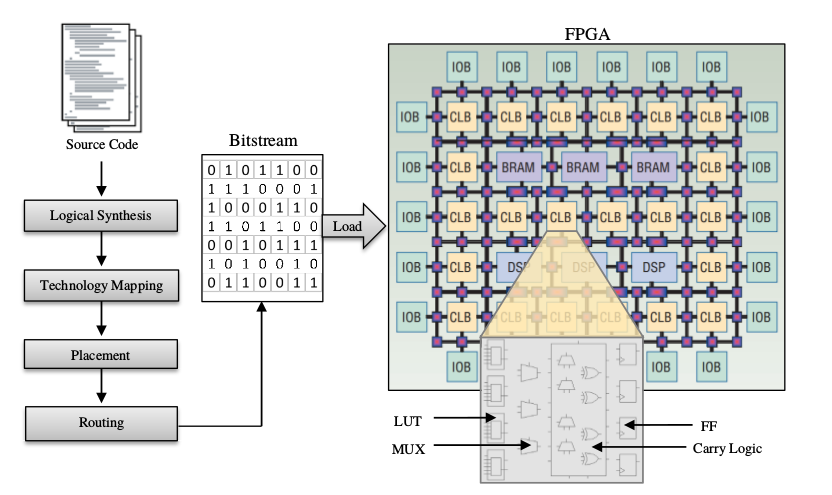
\includegraphics[scale=0.4]{figures/img/FPGA-structure.png}
   \caption{FPGA Structure and Design Flow}
\label{fig:fpga-struct}
\end{figure}





The process starts with the system design written
in a hardware description language (HDL), e.g., VHDL or Verilog. Next, the design is optimized and mapped into the FPGA’s available resources through logical synthesis,
technology mapping, placement, and routing. Finally, the generated bitstream downloaded into the device, and the device starts functioning according to the designer design.
Like any other semiconductor device, FPGAs are sensitive to radiation effects.
Mostly, these effects depend on the technology used to store the configuration data.
Regarding the impact of SEEs on reliability and functionality, FPGAs based on SRAM
technology are a particular class of devices. The foremost concern for SRAM-based FPGAs is
SEUs within the configuration memory. In such devices, this memory may represent more
than 80 percent of the total memory bits, increasing the probability of configuration faults.
Upset configuration bits may change the logic and routing of the implemented system, as
shown in Figure~\ref{fig:seu}, leading to functional failures in an unpredictable way. In contradiction, the primary concern for anti-fuse and flash-based FPGAs is SETs and SEUs within user flip-flops
and block memories. However, the configuration memory blocks of anti-fuse and flash-based
FPGAs offer a relative immunity to SEEs, but these devices have lower logic capacity and
cannot be reprogrammed an unlimited number of times, making SRAM-based FPGAs more
suitable for complex systems requiring frequent reconfiguration and adaptation~\cite{quinn2015validation, violante2004simulation}.

\begin{figure}
 \centering
  \captionsetup{justification=centering}    
   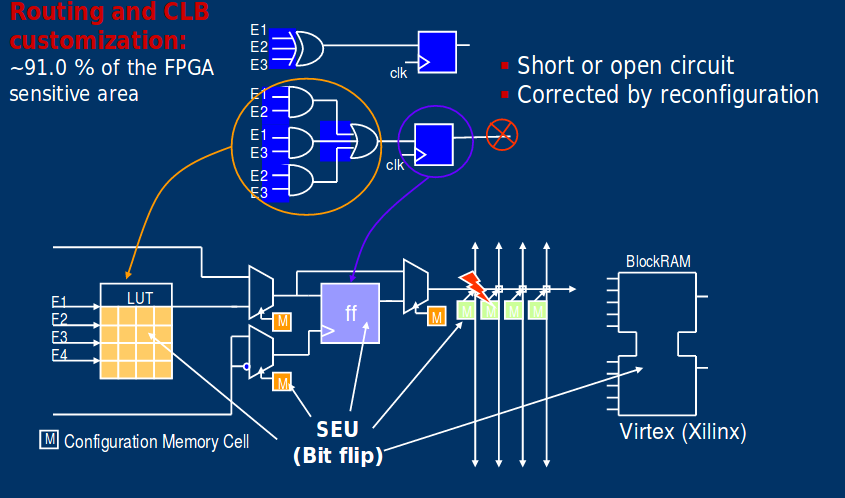
\includegraphics[scale=0.4]{figures/img/seu.png}
   \caption{Upset FPGA configuration bits may change the logic and routing.}
\label{fig:seu}
\end{figure}


\section{Neutron Effects on Electronics}

\section{Fault Injection}

As we discussed before, SRAM-based FPGAs are particularly sensitive to SEUs. The configuration memory is the most sensitive part, by changing the configuration memory, may affect the overall functionality of the system. The work have done so far deal the SEU effects on FPGAs, combines the simulation, radiation, and emulation testing~\cite{quinn2015validation, violante2004simulation, hobeika2014multi, robache2013methodology, quinn2015using, souari2015optimization}. These papers described how they make the faulty behavior of the system to build an accurate representation of the system. The work presented in~\cite{quinn2015using} described the benchmark that can be used for the reliability and radiation effects study on FPGAs and microprocessors. FPGAs offer high densities and run-time programmability facility make inconvenient to use in the aerospace domain. But, FPGAs are sensitive to high-energy ions.  We need to study the sensitivity of SRAM-based FPGAs to heavy ions that show the suitability and analysis of effects of radiation on FPGAs when employed in space, e.g., usage of FPGAs in aircraft. The work presented in~\cite{hobeika2014multi} investigate the sensitivity of SRAM-based FPGAs devices not only for the simulation-based approach but also used emulation and radiation testing for evaluating the effects of SEUs. The work presented in~\cite{souari2015optimization} described the fault injection emulation in Xilinx FPGA based on the identification of critical configuration bits. Based on SRAM-based FPGAs, two aspects can be considered:

\begin{itemize}


\item SEUs may alter the contents of a register in the data path, or the content of the state register.
\item SEUS may alter the content of the configuration memory.

\end{itemize}



\subsection{Simulation}

The work presented in~\cite{robache2013methodology} discuss the fault simulation, fault emulation, and radiation testing. Starting from the simulation, I can interrogate how the authors used the concept of signatures to capture and reproduce the faulty behavior due to SEUs very early in the design process.
Radiation testing is an expensive approach and requires a state-of-the-art facility. The alternative to the radiation testing is the fault-injection approach.  The work presented in~\cite{hobeika2014multi} described the concept of faulty behavior signature. The work demonstrates how faulty behavior signatures allow building high-level models, e.g., high-level faulty model, i.e., Simulink, that reflects the faulty behavior of a combinational circuit represented at gate-level  (injected with one fault arbitrarily selected from a fault list). The main contribution of this work is to capture the effects of radiations on a circuit modeled at a low abstraction level and then abstract it to a  higher level. This challenge can be accomplished by introducing the concept of faulty behavior signature.  The fault injection tool that is used named - LIFTING.  The purpose of this tool is to study the effects of different types of faults on a circuit at gate-level. The tool used the stuck-at 0 and 1 are injected in each node of the design. The LIFTING is a simulation-based gate-level fault injection tool that used the circuit netlist file, e.g.  *.v file, input test vectors, and fault parameters as inputs produced two output files. The one is the golden report and the second consist of fault injection report. These two outputs are used to generate the signatures.  The signature represents the compressed faulty behavior of the circuit. The signatures consist of arrays of errors and their probabilities of occurrence. The signatures are either arithmetic or logic.  The third step is to make a high-level model that corresponds the low-level circuit. The work presented in this paper helps to make a faulty block with Simulink that reads a signature and generates errors according to the distribution.

\subsection{Emulation}
The emulation of SEUs in an FPGA is done by flipping the bit in the configuration memory. The emulation can be done by using the IP provided by the Xilinx named - LogiCORE. The work adopted the emulation work also proposed in the~\cite{hobeika2013flight}.  The work described a completed automated methodology to emulate SEUs on an FPGA efficiently. The authors used the reconfigurable flight control system based on a reference adaptive control model. The difference between the work presented in~\cite{hobeika2014multi} and~\cite{hobeika2013flight} is that; in~\cite{hobeika2013flight} the authors used the flight control system that is based on a linear plant model. Whereas, in~\cite{hobeika2014multi}the emulation is performed on the circuits (adder and multiplier). The work presented in~\cite{hobeika2014multi} used the SEU controller. The emulation is the four step process.

\begin{itemize}

\item Identification of an emulation zone.
\item Fault list generation.
\item SEU emulation.
\item Result Analysis.

\end{itemize}



The identification of an emulation zone used the concept of the essential bits which can be extracted by the Xilinx BitGen command. For example, 253227 bits are identified as the total essential bits in~\cite{hobeika2013flight}, among them, 57464 belongs to the interested essential bits. The step is used to minimize the time because an FPGA device contains millions of configurable bits, emulating a bit flip for every cell would be time-consuming. BitGen gives only the essential bits; that
considered critical bits. The second step generates the fault list. This action creates a list of the corresponding bit addresses (exact bit position to be emulated).  For example, authors observed 7000 emulation requests in~\cite{hobeika2013flight}.  The third step used auto-correct mode in which one bit is flipped at a time and the detect-only mode  (bit flips accumulation possible) where bits are flipped without correction. In the final step, an in-house script is used to characterize and quantify the design sensitivity to SEUs. This script is used to compare the results with the faulty one and fault-free. Authors observed 638 total number of failure in~\cite{hobeika2013flight}. Similarly, authors observed 80384 essential bits among them 2454 are considered as the interested ones for the adder circuit, for multiplier interested essential bits are 1314 among 92337 total essential bits.
The emulation can be performed on the Virtex 5. The 16-bit adder and  8-bit-by-8-bit multiplier are used as a testing circuit. The signatures are recorded in the accumulation mode. And, the estimation of the critical bits performed in the auto-correct mode.
The Emulation setup presented in~\cite{souari2015optimization} adopted the approach for the estimation by fault injection based on the sensitivity. Authors proposed the method in which fault are injected based on the specific bits configurations defined according to their contents and the type of FPGA resources. This new approach outperformed the traditional random fault injection with speed up factors to two orders of magnitude. This fault injection method based on the prioritizing specific subsets of configuration bits. These configuration bits are classified with the statistical analysis according to their values (0 or 1, and 2). The SEU controller a macro developed by Xilinx assuring fault injection, detection, and correction is used a fault injection engine in their experiments. The fault injection is prioritized using the following three steps:

\begin{itemize}

\item   {Classification of the configuration bits into subsets.
        a.  Bits set to 1/0 of LUT.
        b. Bits set to 1/0 configuring other than LUT.
        c. Bits set to 1/0 configuring other resources not identified as  potentially critical by bitgen.}
        
        
\item  {Estimating the number of critical bits of the set by randomly injecting faults in the bits of each set. This method helps to find the most critical zones of the FPGA.}

\item {Prioritized the fault injection in the identified (step-2) most critical zones.
These classification steps are done with the help of EBC and EBD files provided by the bitgen. The experimental results presented in [5] evaluated the SEU sensitiveness as well as bitgen efficiency. The results are evaluated between random fault injection with different prioritized bit subsets.  The first observation authors concluded - the bitgen did not accurately identify all the critical bits meaning the bitgen limitations. Second authors did the prioritizing the most sensitive subset. It would involve exhaustive fault injection. The authors used fault injection to get an estimated number of critical bits as well as the related estimation error. They used the term critical bit error estimate (CBEE). The authors claimed the CBEE observed for the random approach is higher than the observed under the bits subsets.  The ratio of observed critical bits (ROCB) observed for the random injection is far less than the different bits subsets.}



\end{itemize}



\subsection{Radiation testing}
The hardware setup consists of two Artix-7 board. Board A used as a reference and board- B is subjected to radiations. The board-A is not bombarded, and it hosted the counters, reference design error detection and signature computation, memories to store signatures and communication controller. A total 20 runs performed on the adder and 14 on the multipliers. Arithmetic errors for both approached DSP and LUT are observed (151 vs. 291 for DSP). This is due to DSP strategy; SEUs can add registers in the data path, leading to the sequential type of errors. The authors in this work compare the results from the fault simulation, fault emulation, and radiation testing. The purpose is to express as signatures, intended to reproduce the faulty behavior. They showed that simulation and emulation based signatures could contain the same error values as obtained with radiation but their probability of occurrence could significantly different. The arithmetic signature for TRIUMF to emulation is 85.3 % for adder and 84.8% for the multiplier. Similarly, the matching with the simulation of adder and multiplier with TRIUMF is 84.8 % and 100 % respectively.


\section{Fault Models}
\subsection{Stuck-at Fault Model}
\subsection{Functional Fault Model}
\subsection{Open Fault}
\subsection{Stuck-On and Stuck-Off}


\section{Faults Behavioural Modeling}



%\subsection{Benchmark for Radiation Testing}
The suitable selection of the benchmark for the radiation testing of microprocessor and FPGAs is a recently topic of ongoing research. The benchmarks are used to evaluate the performance under different architectures, technology, and compiler. There is no such standard benchmark employed to study microprocessor and FPGAs under the effects of radiations; make it difficult to assess the changes in fabrication technology, architecture, and circuitry. The work presented in~\cite{quinn2015using}described the software and hardware benchmark under the neutron test data. The unavailability of the such a benchmark for testing because radiation hardness assurance techniques are applied only to circuit layouts or manufacturing process. There is no standard test circuits available, researcher, used flip-flop or D-latches to compare their results. In recent years, radiation effects community shown interest to develop a standard set of circuits that include complex and realistic algorithms and can be adapted to different FPGAs.  Currently, without standard benchmark researcher used the following approach for testing:

\begin{itemize}


\item Homemade Design.
\item Circuits from Opencore.
\item Proprietary designs.
\end{itemize}


The problem with this approach as no two organizations used the same set of codes or circuits, difficult to make the comparison. There is a need for collaboration to make a suitable set of benchmark for reliability application and study the effects of radiation under the same conditions. The criteria used to set a standard benchmark including:

Repeatability of benchmark tests.
A representative of deployed computing workload.
Availability of fixed input vectors.
Cross-platform implementation.
The ability to repeat test itself is an important part of the standardized testing. By repeating the algorithms, the input test vector, the compilation, the synthesis setting help researchers to have the enough information. It is necessary to provide a wide variety of realistic algorithms so that the system can be tested as likely to the realistic application. Defining the input test vector is an essential step because many hardware errors can be observed under the specific set of the test vector. It is an open question which input test vector should be adopted, under the specific set of criteria. Finally, the implementation of the algorithms in portable languages help to use the same set of codes on the different platform. For example, assembly language for the microprocessors limit the ability to compare and port codes on the different platform. But the hardware benchmark developed in VHDL can ease the problem; the same circuit can be ported to any FPGA.

\textbf{FPGA Radiation Benchmark}

The FPGA benchmark mentioned in this paper is ITC'99 which is well defined ATPG benchmark. This benchmark meets all the requirements, e.g., realistic algorithms, input vectors, scalability, and portability. The circuits are implemented in the HDL so that it can be ported to different FPGAs. The first 15 circuits from the ITC'99 are adopted for the benchmark as shown in Table I.

\textbf{Software Radiation Benchmark}

The software radiation benchmark is harder to design than the FPGA radiation benchmark. The development of the standard set of algorithm that can be ported on different architectures would be a challenging task e.g., porting an algorithm to 16-bit microcontroller to GPU. The authors are interested in the software benchmark where the computational load can be divided into the parallel processes or run on a single core. The commonly used software benchmark comprises of fast fourier transform, matrix multiplication and quick-sort algorithm as they are commonly used in many applications and useful for the evaluating the reliability of parallel processors. The software benchmark comprises the following code.

\begin{itemize}
\item AES-128;
\item Cache test;
\item FFT;
\item Hotspot;
\item HPCCG;
\item Matrix Multiply;
\item Quicksort
\end{itemize}





\textbf{Radiation Testing}
The radiation testing is completed at Los Almos Neutron Science Center (LANSCE). The results are provided for the microcontroller, ARM cores, GPUs, and FPGAs. The B13 from ITC99 is used under the hardware benchmark suite; Virtex- 5 is used as a hardware platform. They also provide the result for the mitigation. For mitigation, they used X-TMR and VERI-Place. The failure in time (FIT) are decreased under mitigation, but the overhead is increased (circuit area increased).

\textbf{Hardware Benchmark Testing}
For the hardware radiation testing the authors used the B13 from the ITC’99 benchmark suite. The circuit is too small so it can be replicated 30 times, the implementation is done on the Virtex-5. Both unmitigated and mitigated version are tested. The results for FPGA radiation reports SDCs from the mitigated circuits normalized to the SDCs from the unmitigated circuits. Mitigated circuits are likely to fail at three times the rate of the unmitigated circuit, because of the increased size of the circuit from the mitigation process. The mitigated circuit cross-section is three times larger than an unmitigated circuit when SEUs accumulate. The authors conclude; the VERI-place mitigated circuits perform better than the X-TMR mitigated circuits.

\textbf{Software Benchmark Testing}
Software benchmark radiation testing is done on the flash-based microcontroller,  a ferroelectric-memory-based microcontroller, two ARMs, and GPUs. These components are tested with both mitigated and unmitigated codes. The results reported in the paper for two different microcontroller and two ARMs cores. For microprocessors: these microprocessors have very small SRAM the FITs are very small. In some cases, there is no error from the code during many days of testing. They also implemented the matrix multiplication, FFT, and Hotspot on NVIDIA K20 GPU and applied mitigation methods (ECC, ABFT, and DWC).  The purpose is to see the effect of overhead by applying the mitigation technique; the overhead has been increased as compared it with the unhardened configuration.
In short, the work presented in [3] evaluate a common set of hardware and software benchmarks to evaluate reliability and radiation effects on FPGA and microprocessors.





%\section{Fault-detection, mitigation and correction in the FPGA }


The impact of SEUs on SRAM FPGA devices has been studied in~\cite{bellato2004evaluating}. Many  techniques  have  been  proposed to provide highly reliable FPGA devices, e.g. radiation-hardened FPGAs~\cite{rockett2007radiation}, in-order to lower the effect of radiation-induced SEUs. However, radiation-hardened  SRAM  FPGAs  typically have  a  low  density, and  they  only  may  lower  the  probability of SEUs to occur but  not  completely avoid  them. Therefore, non radiation-hardened FPGAs, like the  Xilinx Kintex-7, are evaluated under a harsh radiation  environment~\cite{wirthlin2014soft}. Even on radiation-hardened FPGAs, the SEU rate in a low-earth orbit flight experiment can be up to 16 events per day~\cite{quinn2012orbit}. A wide  variety  of  SEU  fault  mitigation  techniques  for SRAM-based  FPGAs  have  been  proposed  during  the  past years. These techniques can be categorized into module redundancy techniques such as triple modular redundancy (TMR)~\cite{lyons1962use} and techniques that use scrubbing of the FPGA configuration memory~\cite{heiner2009fpga}. Also the combination of  both techniques has been shown to be able to increase the reliability of FPGA modules significantly ~\cite{ostler2009sram}. FPGA-based TMR approaches replicate a given module which shall be protected either statically or dynamically~\cite{angermeier2011runtime}. The different granularities of voted replicas  are evaluated in~\cite{bolchini2007tmr}. However, no upset rates and consequential no reliability figures are provided. Nevertheless, TMR techniques are  known to often cause an excessive and unacceptable overhead in terms of power  consumption and area. Since the intensity of a cosmic rays is not constant but may vary over several magnitudes depending on the solar activity, a worst-case radiation protection is far too expensive in most cases. A self-adaptive system is proposed in~\cite{glein2014self}, which monitors the current SEU rate and exploits the opportunity of partial reconfiguration of FPGAs to implement redundancy such as TMR on demand. 

Memory scrubbing is a well-known correction technique for the configuration memory of SRAM-based FPGAs. It consists on re-writing the configuration memory after the FPGA is configured to restore its original content. It is often a transparent operation for the running application. This is possible because modern FPGAs offer a dynamic partial reconfiguration (DPR) feature. The circuit that enables the scrubbing is commonly named scrubber. Additionally, readback is the process of reading the configuration memory of the FPGA after it is configured. Both processes (readback and scrubbing) can be used to implement different scrubbing methodologies as shown in~\cite{herrera2013design}. Scrubbing can be implemented using an internal or external interface as shown in~\cite{berg2008effectiveness}. When external interface is used, the scrubbing logic is implemented outside the FPGA. In the case of Xilinx FPGAs several external interfaces are available; however, the Select MAP interface has the highest data throughput. On the other hand, there is only one internal interface named ICAP~\cite{xilinx}. This internal interface can be accessed from the reconfigurable logic of the FPGA and it is a replica of the Select MAP interface. Also scrubbers can be implemented in software or hardware. The scrubbing process can be implemented using a microprocessor with the advantage of a high flexibility to implement different complex scrubbing methodologies but with lower configuration speeds and lower energy efficiency.

\section{Combinational Testing Vs. Sequential Testing}

\subsection{Built-In Self-Test (BIST)}
\subsection{All Test Pattern Generator (ATPG)}
\subsection{Scan Chain Testing}

\section{Conclusion}
The work done so far [1, 2, 3, 4, and 5] evaluated and quantified the SEU effects by performing simulation, emulation, and radiation on an SRAM-based FPGA. Implemented a design, observed its faulty behavior in the presence of SEU and extracted the corresponding fault model. Presented an automated methodology to efficiently used the SEU controller. Discussed the fault injection on the specific subsets rather than random and discussed the selection of the suitable benchmark for FPGA and microprocessor radiations. 




%%% Local Variables:
%%% mode: latex
%%% TeX-master: "../Document"
%%% End:
